\documentclass[../TDT4.tex]{subfiles}%

\begin{document}
\section[s]"2"{Possibilité d'un cycle}
\enonce{%
	On raisonne sur une quantité de matière $n = \SI{1}{mol}$ de gaz parfait qui
	subit la succession de transformations (idéalisées) suivantes~:
	\begin{itemize}
		\item[b]{AB}: détente isotherme de $P\ind{A} = \SI{2}{bar}$ et $T\ind{A} =
			\SI{300}{K}$, jusqu'à $P\ind{B} = \SI{1}{bar}$ en restant en contact avec
		un thermostat de température $T_0 = T\ind{A}$~;
		\item[b]{BC}: évolution isobare jusqu'à $V\ind{C} = \SI{20.5}{L}$, toujours
		en restant en contact avec le thermostat à $T_0$~;
		\item[b]{CA}: compression adiabatique réversible jusqu'à revenir à l'état A.
	\end{itemize}
	On suppose le gaz diatomique.
}%

\QR{%
	Quel est le coefficient adiabatique~? Calculer les coordonnées des points puis
	représenter ce cycle en diagramme de \textsc{Watt} $(P,V)$.
}{%
	\noindent
	\begin{minipage}[t]{.68\linewidth}
		On a un gaz diatomique, donc $\boxed{\gamma = \frac{7}{5}}$.
		\begin{itemize}
			\item
			      \leftcenters{%
				      \textbf{A}~:
			      }{%
				      $V\ind{A} = \frac{nRT\ind{A}}{P\ind{A}} = \SI{12}{L}$
			      }%
			\item
			      \leftcenters{%
				      \textbf{B}~: isoT $\Ra T_B = T\ind{A} \Ra$
			      }{%
				      $V\ind{B} = \frac{nRT\ind{A}}{P_B} = \SI{25}{L}$
			      }%
			      \item[b]{C}: déjà connues.
			      \item[b]{Tracé}: AB isotherme en hyperbole ($P \propto 1/V$), AC
			      adiabatique donc plus penchée ($P \propto 1/V^{\gamma}$ avec
			      $\gamma>1$).
		\end{itemize}
	\end{minipage}
	\hfill
	\begin{minipage}[t]{.30\linewidth}
		\vspace{0pt}
		\begin{center}
			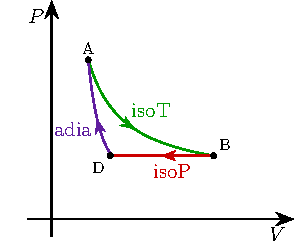
\includegraphics[width=\linewidth]{E4_PV_cycle}
		\end{center}
	\end{minipage}
}%
\QR{%
	À partir du diagramme, déterminer le signe du travail total des forces de
	pression au cours du cycle. En déduire s'il s'agit d'un cycle moteur ou d'un
	cycle récepteur.
}{%
	En valeur absolue, le travail des forces de pression au cours d'une
	transformation correspond à l'aire sous la courbe représentant cette
	transformation dans le diagramme de Watt. Il est positif si le volume diminue
	au cours de la transformation et négatif s'il augmente. Ici, les deux
	transformations BC et CA comptent positivement et la transformation AB compte
	négativement. On voit sur le diagramme que l'aire sous AB est supérieure à la
	somme des aires sous BC et CA~: \textbf{cycle en sens horaire} donc le
	\textbf{travail des forces de pression est globalement négatif sur l'ensemble
		du cycle}. Cela indique que le système fournit effectivement du travail à
	l'extérieur~: il s'agit d'\textbf{un moteur}.
}%
\QR{%
	Déterminer l'entropie créée entre A et B. Commenter.
}{%
	La transformation AB est isotherme, donc on utilise une expression de
	$\Delta{S}\ind{AB}$ qui implique $T$ pour l'éliminer. Par exemple,
	\[
		\Delta{S}\ind{AB} = nR \ln \frac{P\ind{A}}{P\ind{B}}
	\]
	De plus, pour avoir $Q\ind{AB}$ et donc $S\ind{ech,AB}$, on a
	\begin{align*}
		\beforetext{Premier principe}
		\Delta{U}\ind{AB}      & = W\ind{AB} + Q\ind{AB}
		\\\beforetext{Isotherme donc}
		C_V \Delta{T} = 0      & = W\ind{AB} + Q\ind{AB}
		\\\beforetext{Calcul de $W$}
		W\ind{AB}              & = -\int_{A}^{B} P\ind{ext} \dd{V}
		\\\beforetext{Si quasi-statique}
		\Lra
		W\ind{AB}              & = - \int_{A}^{B} P \dd{V}
		\\\beforetext{$P = nRT/V$}
		\Lra
		W\ind{AB}              & = - \int_{A}^{B} nRT \frac{\dd{V}}{V}
		\\\beforetext{$T = \cte$}
		\Lra
		W\ind{AB}              & = - nRT\ind{A} \ln \frac{V\ind{B}}{V\ind{A}}
		\\\beforetext{$V\ind{B}/V\ind{A} = P\ind{A}/P\ind{B}$}
		\Lra
		-W\ind{AB} = Q\ind{AB} & = -nRT\ind{A} \ln \frac{P\ind{B}}{P\ind{A}}
		\\\beforetext{$S\ind{ech,AB}$ thermostat}
		\Ra
		S\ind{ech,AB}          & = \frac{Q\ind{AB}}{T_0} = nR \ln \frac{P\ind{B}}{P\ind{A}}
		\\\Lra
		\Delta{S}\ind{AB}      & = S\ind{ech,AB} + 0
		\\\Lra
		\Aboxed{S\ind{cr,AB}   & = 0}
	\end{align*}
	La \textbf{transformation AB est donc réversible}.
}%
\QR{%
	Calculer la température en C, le travail $W\ind{BC}$ et le transfert thermique
	$Q\ind{BC}$ reçus par le gaz au cours de la transformation BC. En déduire
	l'entropie échangée avec le thermostat ainsi que l'entropie créée. Conclure~:
	le cycle proposé est-il réalisable~? Le cycle inverse l'est-il~?
}{%
	D'après l'équation d'état du gaz parfait,
	\[
		\boxed{T\ind{C} = \frac{P\ind{B}V\ind{C}}{nR}}
		\Ra
		\xul{T\ind{C} = \SI{2.5e2}{K}}
	\]
	Transformation isobare, donc
	\[
		\boxed{W\ind{BC} = -P\ind{B} (V\ind{C} - V\ind{B})}
		\Ra
		\xul{W\ind{BC} = \SI{4.4e2}{J}}
	\]
	On a $Q\ind{BC}$ avec le premier principe enthalpique~:
	\begin{align*}
		Q\ind{BC} & = \Delta{H}\ind{BC} = C_P (T\ind{C} - T\ind{B})
		\\\Lra
		\Aboxed{
		Q\ind{BC} & =
			\frac{\gamma nR}{\gamma-1} \left( T\ind{C} - T\ind{B} \right)
		}
		\\\Ra
		\makebox[0pt][l]{$\phantom{\AN}\xul{\phantom{Q\ind{BC} = \SI{-1.6}{kJ}}}$}
		\AN
		Q\ind{BC} & = \SI{-1.6}{kJ}
	\end{align*}
	Donc pour l'entropie échangée~:
	\[
		\boxed{S\ind{ech,BC} = \frac{Q\ind{BC}}{T_0}}
		\Ra
		\xul{S\ind{ech,BC} = \SI{-5.2}{J.K^{-1}}}
	\]
	Pour calculer l'entropie créée, il faut d'abord calculer la variation
	d'entropie du gaz entre B et C, ce qui se fait avec les expressions données.
	Comme la transformation est isobare, le plus astucieux est d'utiliser une
	expression dépendant de $P$ puisque les termes associés se composent alors. On
	en déduit
	\[
		\boxed{
			\Delta{S}\ind{BC} = \frac{\gamma nR}{\gamma-1}\ln \frac{T\ind{C}}{T\ind{B}}
		}
		\Ra
		\xul{\Delta{S}\ind{BC} = \SI{-5.7}{J.K^{-1}}}
	\]
	D'où l'entropie créée
	\[
		\boxed{S\ind{cr,BC} = \Delta{S}\ind{BC} - S\ind{ech,BC}}
		\Ra
		\xul{S\ind{cr,BC} = \SI{-0.5}{J.K^{-1}}} < 0
	\]
	L'entropie créée au cours de l'étape BC serait donc négative, ce qui est
	\textbf{absolument impossible}~: le cycle proposé est donc
	\textbf{irréalisable}. En revanche, le \textbf{cycle inverse est possible},
	car deux transformations sont réversibles et la troisième aurait une création
	d'entropie, ce qui est permis et décrit par le second principe.
}%

\end{document}
